\begin{frame}
 \frametitle{Cylindrical coordinates}
\begin{columns}
\column{0.4\textwidth}
%
  \psfrag{P}{$P$}
  \psfrag{O}{$O$}  
  \psfrag{xp}{$x_P$} 
  \psfrag{yp}{$y_P$} 
  \psfrag{zp}{$z_P$}     
  \psfrag{rp}{$r_P$}
  \psfrag{thp}{$\theta_P$}
  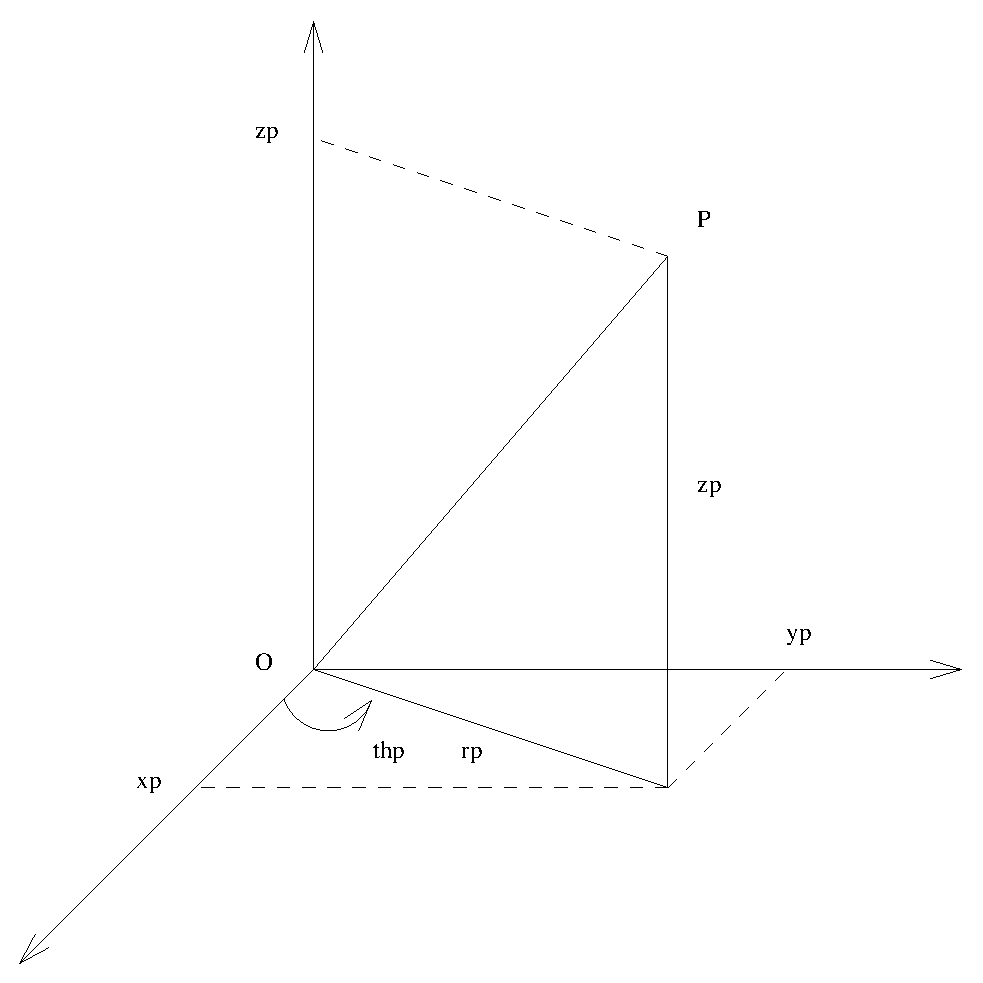
\includegraphics[height=2in]{../../modules/coordinate-systems/pictures/cylindrical_coordinates.eps}
  %\caption{Cylindrical coordinates}
  %\label{fig:cylindrical-coordinates}
%
\column{0.6\textwidth}
$$P(x,y,z) \Longleftrightarrow P(r, \theta, z)$$

\begin{itemize}
    \item Polar in $Oxy$ -- $(r, \theta)$;
    \item Rectangular in $Orz$ -- $(r, z)$.
\end{itemize}
\end{columns}

\end{frame}

\begin{frame}

\begin{columns}
\column{0.4\textwidth}
  \psfrag{P}{$P$}
  \psfrag{O}{$O$}  
  \psfrag{xp}{$x_P$} 
  \psfrag{yp}{$y_P$} 
  \psfrag{zp}{$z_P$}     
  \psfrag{rp}{$r_P$}
  \psfrag{thp}{$\theta_P$}
  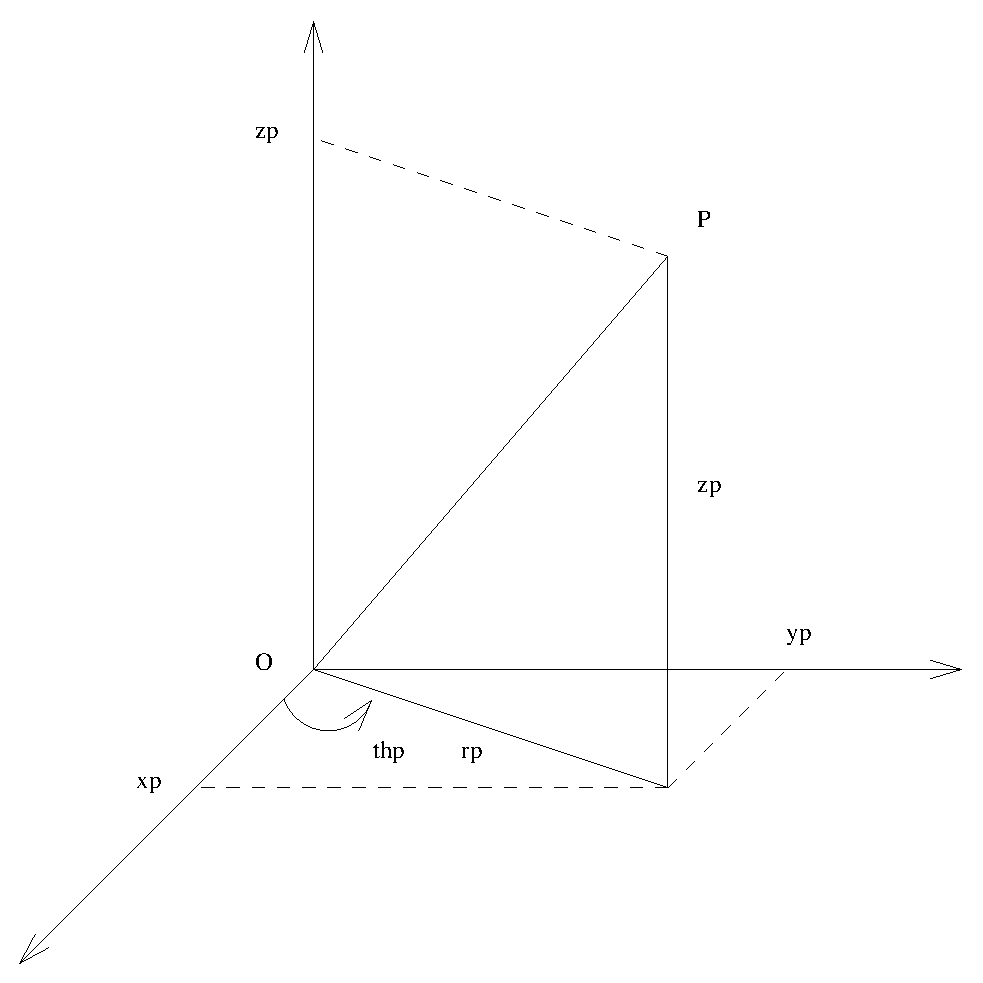
\includegraphics[height=2in]{../../modules/coordinate-systems/pictures/cylindrical_coordinates.eps}
  %\caption{Cylindrical coordinates}
  %\label{fig:cylindrical-coordinates}
%
\column{0.6\textwidth}
To transform cylindrical to rectangular coordinates:\pause
$$x=r\cos\theta \quad , \quad y = r\sin\theta \quad , \quad z_{r} = z_{c}$$

Rectangular to cylindrical:\pause
$$r= \sqrt{x^2+y^2} \quad , \quad z_{c}=z_{r}$$
$$\cos\theta = \frac{x}{r} \quad , \quad \sin\theta = \frac{y}{r}\; .$$
\end{columns}
\end{frame}

\begin{frame}
\frametitle{Constant Coordinate Sets}
\begin{columns}
\column{0.4\textwidth}
  \psfrag{P}{$P$}
  \psfrag{O}{$O$}  
  \psfrag{xp}{$x_P$} 
  \psfrag{yp}{$y_P$} 
  \psfrag{zp}{$z_P$}     
  \psfrag{rp}{$r_P$}
  \psfrag{thp}{$\theta_P$}
  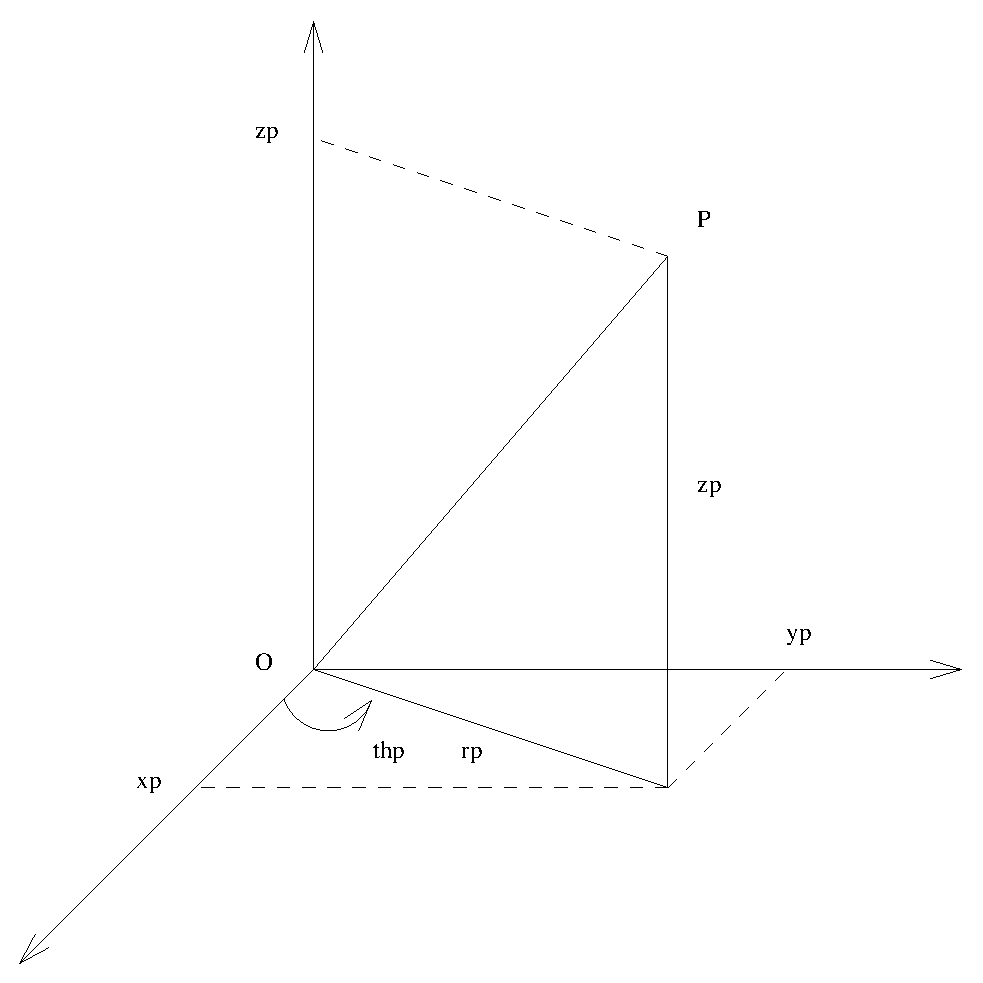
\includegraphics[height=2in]{../../modules/coordinate-systems/pictures/cylindrical_coordinates.eps}
\column{0.6\textwidth}

Surfaces:
\begin{itemize}
  \item $r$ constant \pause$\to$ vertical cylinder;
  \item $\theta$ constant \pause$\to$ vertical half plane;
  \item $z$ constant \pause$\to$ horizontal plane.\pause
\end{itemize}
%
Curves:
\begin{itemize}
 \item $\theta, z$ constant \pause$\to$ horizontal ray;
\item $r, z$ constant \pause$\to$ horizontal circle;
\item $r, \theta$ constant \pause$\to$ vertical line.
\end{itemize}
\end{columns}
\end{frame}